\documentclass[a4paper]{article}

\usepackage[english]{babel}
\usepackage[utf8]{inputenc}
\usepackage{amsfonts}
\usepackage{amssymb}
\usepackage{amsmath,amsfonts}
\usepackage{graphicx}
\usepackage[colorinlistoftodos]{todonotes}
\usepackage{titling}
\usepackage{listings}
\usepackage[T1]{fontenc}
\usepackage{array,multirow,makecell}
\setcellgapes{1pt}
\makegapedcells
\newcolumntype{R}[1]{>{\raggedleft\arraybackslash }b{#1}}
\newcolumntype{L}[1]{>{\raggedright\arraybackslash }b{#1}}
\newcolumntype{C}[1]{>{\centering\arraybackslash }b{#1}}

\newcommand{\subtitle}[1]{%
  \posttitle{%
    \par\end{center}
    \begin{center}\large#1\end{center}
    \vskip0.5em}%
}
\lstset{%
  basicstyle=\scriptsize\sffamily,%
  commentstyle=\footnotesize\ttfamily,%
  frameround=trBL,
  frame=single,
  breaklines=true,
  showstringspaces=false,
  numbers=left,
  numberstyle=\tiny,
  numbersep=10pt,
  keywordstyle=\bf
}





%%%%%%%%%%%%%%%%%%%%%%%%%%%%%%%%%%%%%%%%%%%%%%%%%%%%
% Raport Headers:
%%%%%%%%%%%%%%%%%%%%%%%%%%%%%%%%%%%%%%%%%%%%%%%%%%%%
\title{ISP: Computer exercise 5\\CE04G02T05}
\author{PASHEVICH Alexander \and SID-LAKHDAR Riyane}
\date{25/11/2015}

\begin{document}
% Beginning serious stuff.


\maketitle


\begin{abstract}
The problem of image finding is one of the most important in Image Analysis. The template matching technique is one of the most straightforward and understandable methods to achieve this goal. In this report we would like to introduce this technique by at first proving some theoretical material and showing the application of it to 1D and 2D signals.\\
For the seek of comprehension, a discrete finite length signal of N samples will be considered as infinite by extending it with zeros or by using an N-periodic shifting.
\end{abstract}

%\tableofcontents



\section{Introduction}
To match template we have to think about some measurement of metrics that can be used. In the following paragraphs we will introduce such metrics and show its link with convolution. After we do it, we will apply this technique on simple impulse signal and shifted periodic signal with noise. Once we are done with the 1D signals, we will introduce results obtained while working with images.



\section{Material \& Methods}
    \subsection{Descriptions: pattern matching tools}
        \subsubsection{Evaluate the difference between signals}
A signal s with N samples may be considered as a vector into an N-dimensional "Euclidean space".   In this representation, each sample i of s would be the projection of the vector s on the $i^{th}$ base vector of the Euclidean space.   Thus, this samples of s are encoding the magnitude $||s||$ and the direction $\theta$ of the vector.\\

Using this representation, we can characterize the difference between two vectors by using the direct angle between them directions.   The more this vectors would be different, the more the distance between them directions would be big.   This property is guaranteed by the following indicator M:
\begin{equation*}
\begin{aligned}
	M(s_{0}, s_{1})	&= \frac{|<s_{0}, s_{1}>|}{||s_{0}|| . ||s_{1}||}\\
    				&= \frac{||s_{0}|| . ||s_{1}|| * cos(\theta)}{||s_{0}|| . ||s_{1}||} \mbox{ where }\theta \mbox{ is the direct angle between } s_{0} \mbox{ and } s_{1}\\
	M(s_{0}, s_{1})	&= cos(\theta)
\end{aligned}
\end{equation*}






	      \subsubsection{Cross correlation operation}
Let u and v two discrete real signals.   The cross correlation between this two signals is defined for each index l by $C_{uv}[l] = \sum_{k=-\infty}^{+\infty}{u[k+l] v[k]}$.
This representation considers for each sample $k$ of $v$ the sample $k+l$ of $u$. It is a forward computing.  An equivalent backward computing formula may be deduced by:
\begin{equation*}
\begin{aligned}
	C_{uv}[l]&= \sum_{k=-\infty}^{+\infty}{u[k+l] v[k]} \\
	 		&= \sum_{k'=-\infty}^{+\infty}{u[k'] v[k'-l]} \\
\end{aligned}
\end{equation*}
Where $k' = k+l$ for each fixed l.





			\subsubsection{Energy of a signal}
In this section, we will consider a signal $X$ defined through its N finite samples $\{X[0], X[1], ..., X[N-1]\}$ ($N \in \mathbb{N}$).   We also consider the signal $x_{l}$ defined for each $l \in \mathbb{N}$ as $x_{l} = x[k+l]$.\\

Thanks to this signals, we define the energy of a signal s as $E(s) = \sum_{k=0}^{N-1}{(x[k])^2}$.\\


		\subsubsection{Power of a periodic signal}
Let the signal $period$ a signal with $T_{0}$ samples containing one period of a T0-periodic sine function.  This signal may be formally defined $\forall k \in [0, T_{0}]$ as $period[k] = sin(\frac{2 \pi k}{T_{0}})$.\\ 
The power of such a signal is defined as $P_{signal} = \frac{1}{T_{0}} * \sum_{k=0}^{T_{0}-1}{period[k]^2}$.\\



    \subsection{Analysis}
			\subsubsection{Physical representation of the energy and its effects}
First of all, let illustrate the physical representation of this energy.\\
An N-samples signal s may be represented as an N-dimensional vector within an N-dimensional Euclidean space.   The magnitude of this vector is $ \sqrt{\sum_{k=0}^{N-1}{s[k]^2}}$.   
Thus, the energy of a signal s is the square of its magnitude.\\

Secondly, let focus on the impact of the circular shifting previously defined ($x_{l}$) on the energy of a signal.
For a given strictly positive integer l, the energy of a signal $x_{l}$ is
\begin{equation*}
\begin{aligned}
  E(x_{l})	&= \sum_{k=0}^{N-1}{(x_{l}[k])^2}
		= \sum_{k=0}^{N-1}{(x[k+l])^2}
		= \sum_{k=l}^{N-1+l}{(x[k])^2}\\
		&= \sum_{k=l}^{N-1}{(x[k])^2} + \sum_{k=N}^{N-1+l}{(x[k])^2} \\
		&= \sum_{k=l}^{N-1}{(x[k])^2} + \sum_{k=N}^{N-1+l}{(x[k\mbox{ mod }N])^2} \\
		&= \sum_{k=l}^{N-1}{(x[k])^2} + \sum_{k=0}^{l-1}{(x[k])^2} \mbox{ because } N-1+l \leq 2*N \\
		&= \sum_{k=0}^{N-1}{(x[k])^2}
\end{aligned}
\end{equation*}
Thus, the circular shift of a signal keeps the signal's energy unchanged.







			\subsubsection{Link between correlation and signal's pattern recognition}
Let $X$ an M-samples signal and $S_{T}$ an N-samples signal (with $M \geq N$).   The distance (difference) between $S_{T}$ and a circularly l-shifted sub signal of $X$ of size $N$ is given by the indicator function as:
\begin{equation*}
\label{M_equal_C}
\begin{aligned}
    M(X, S_{T})[l]	&= \frac{|<x_{l}, S_{T}>|}{||x_{l}|| * ||S_{T}|| } \\
    				&= \frac{\sum_{k=-\infty}^{\infty}{x_{l}[k+l]*S_{T}[k]}}{\sqrt{E(x_{l}} * \sqrt{E(S_{T})}}\\
    				&= \sum_{k=-\infty}^{\infty}{(\frac{x_{l}[k+l]}{\sqrt{E(X)}} \frac{S_{T}[k]}{\sqrt{E(S_{T})}})} \mbox{ Because } E(X) \mbox{ and } E(S_{T}) \mbox{ don't depend on } k\\
                    &= \sum_{k=-\infty}^{\infty}{x'_{l}[k+l] * S'_{T}[k]} \mbox{ here we define this new notation $x'_{l}$ and $S'_{T}$} \\
                    &= C_{x'_{l}S'_{T}}
\end{aligned}
\end{equation*}




		\subsubsection{Improving the computation of the power of a signal}
Thanks to the definition of a periodic signal ($P_{signal} = \frac{1}{T_{0}} * \sum_{k=0}^{T_{0}-1}{period[k]^2}$), we can notice that this power is proportional to the energy of the signal.   This definition also shows that T computation are required to compute this power (or energy).\\

Let now see how to use the different symmetry property of the previously defined periodic signal to improve the performance of this computation.
\begin{equation*}
\begin{aligned}
	P_{signal}	&= \frac{1}{T_{0}} * \sum_{k=0}^{T_{0}-1}{sin(\frac{2 \pi k}{T_{0}})^2} \\ 
				&= \frac{1}{T_{0}} * \sum_{k=0}^{T_{0}}{(sin(\frac{2 \pi k}{T_{0}})^2)} - \frac{1}{T_{0}} * sin(\frac{2 \pi T_{0}]}{T_{0}})^2
                = \frac{1}{T_{0}} * \sum_{k=0}^{T_{0}}{sin(\frac{2 \pi k}{T_{0}})^2}\\
                &= \frac{1}{T_{0}} * \sum_{k=0}^{\frac{T_{0}}{2}}{sin(\frac{2 \pi k}{T_{0}})^2 + sin(\frac{2 \pi (T_{0}-k)}{T_{0}})^2} \mbox{\space \space $^($\footnotemark[1]$^)$}\\
                &= \frac{1}{T_{0}} * \sum_{k=0}^{\frac{T_{0}}{2}}{sin(\frac{2 \pi k}{T_{0}})^2 + sin(2\pi - \frac{2 \pi k}{T_{0}})^2}\\
                &= \frac{1}{T_{0}} * \sum_{k=0}^{\frac{T_{0}}{2}}{sin(\frac{2 \pi k}{T_{0}})^2 + sin(\frac{2 \pi k}{T_{0}})^2} \\
                &= \frac{2}{T_{0}} * \sum_{k=0}^{\frac{T_{0}}{2}}{sin(\frac{2 \pi k}{T_{0}})^2}
\end{aligned}
\end{equation*}

\footnotetext[1]{\textbf{$\forall x \in [0, 2\pi], sin(x) = - sin(2\pi - x) $}}

This last simplification comes from the fact that the sin function is anti-symmetric regarding the abscissa axes over a period $\pi$($\forall \alpha \in [0, 2\pi], sin(2\pi - \alpha) = -sin(\alpha)$).   We can use the same reasoning on the property of sin over half a period $\pi$.  The result is:
\begin{equation*}
	P_{signal} = \frac{4}{T_{0}} \sum_{k=0}^{T_{0}/4}{sin(\frac{2\pi}{T_{0}})^2}
\end{equation*}
This formula shows how to use the symmetry properties of this periodic signal to compute its power more efficiently (dividing the computation's time by 4).





\subsubsection{Evaluating the noise impact}
The power previously defined is used to show the impact of a noise signal added to our initial signal.   In this section, we will add to our previously defined periodic signal a Gaussian noise. Then we will use the signal to noise ratio (SNR) to determine the acceptable level of noise that our periodic signal can tolerate.   By tolerate, we mean that the difference between the original and the perturbed signal stays reasonable.\\

Let "$noise$" our Gaussian noise signal and $r_{db}$ the value of the "Signal to Noise Ratio".    Using the definition of the dB SNR, we have:
\begin{equation*}
\begin{aligned}
	10 * log(\frac{P_{signal}}{variance(noise) })	&= r_{db} \\
	log(\frac{P_{signal}}{variance(noise) })		&= \frac{r_{db}}{10} \\
	\frac{P_{signal}}{variance(noise) }				&= 10^{\frac{r_{db}}{10}} \\
	variance(noise)									&= \frac{P_{signal}}{10^{\frac{r_{db}}{10}} } \\
\end{aligned}
\end{equation*}
To show the impact of a noise signal on the initial signal, let take the example of a noise signal which creates a SNR in dB unit of -5dB.   Thanks to the previously computed formula, we have $variance(noise) = \sqrt{10} * P_{signal}$.   Thus, the noise creates a power bigger than the signal's power it self.   So this noise would make the original signal hardly recognizable (at least by our previously defined indicator).






    \subsection{Implementation}
    To check our theoretical results, we have implemented a python program with all the previously defined pattern matching tools.
\begin{figure}[ht!]
\begin{lstlisting}
def energy2D(img):
    e = 0
    for x in range(len(img)):
        for y in range(len(img[0])):
            e += img[x, y] ** 2
    return e
\end{lstlisting}
\caption{Python function to compute the energy of a 2D signal}
\label{energy2D.py}
\end{figure}



We have also designed functions to generate the specific used signals:

\begin{figure}[ht!]
\begin{lstlisting}
def create_impulse_signal(N, a):
    sig = np.zeros(N)
    sig[a] = 1
    return sig

\end{lstlisting}
\caption{Python function to generate an impulse signal}
\label{impulse.py}
\end{figure}


\begin{figure}[ht!]
\begin{lstlisting}
def create_one_period_sin_signal(T0):
    x = np.arange(0, T0)
    return np.sin(2 * np.pi * x / T0)
\end{lstlisting}
\caption{Python function to generate a 1 period sinus function}
\label{one_period_sin_signal.py}
\end{figure}




\begin{figure}[ht!]
\begin{lstlisting}
def create_x(T0, k0, N, SNR):
    sig = create_one_period_sin_signal(T0)
    var = p(sig, T0) / SNR
    noise = np.random.normal(0, scale=var, size=N)
    x = np.zeros(N)
    for k in range(N):
        if k - k0 >= 0 and k - k0 < T0:
            x[k] = sig[k - k0] + noise[k]
        else:
            x[k] = noise[k]
    return x
\end{lstlisting}
\caption{Python function to generate a shifted periodic signal with a Gaussian perturbation}
\label{create_x.py}
\end{figure}















\section{Experiments}
    \subsection{Experimental setup}
    \subsection{Pattern matching in a signal}
    \subsubsection{Analyze the difference between signals}
    Thanks to the indicator M previously defined, we have already defined the difference between two signals as $s_{1}$ and $s_{2}$ as $M(s_{0}, s_{1})	= cos(\theta)$
    where $\theta$ is the direct angle between the two vectors.\\
    Thus, this indicator is high (close to 1) when the directions of the 2 input vectors are close (with an absolute relative angle $|\theta| \in [0, \frac{\pi}{2}[$).\\
    To illustrate this property, let consider the 3 sample signals $x_{1} = \{1, 1, 1\}, x_{2} = \{1, 0, 3\}, x_{3} = \{2, 2, 2\}$.  We have:
    \begin{equation*}
    \begin{aligned}
	    M(x_{1}, x_{2}) &= \frac{1*1 + 1*0 + 1*3}{\sqrt{1^2 + 1^2 + 1^2} + \sqrt{1^2 + 0^2 + 3^2}} = 0.73\\
	    M(x_{1}, x_{3}) &= \frac{1*2 + 1*2 + 1*2}{\sqrt{1^2 + 1^2 + 1^2} + \sqrt{2^2 + 2^2 + 2^2}} = 1
    \end{aligned}
    \end{equation*}

    Thus, $x_{2}$ is closes to $x_{1}$ than $x_{3}$.




	\subsubsection{Matching a simple impulse}
    In this section, we will consider an impulse signal x with 100 samples and the non-zero sample at index 50. We will also consider the impulse signal $s_{T}$ with 40 samples and the non-zero sample at index 20.   Thanks to the python code defined in the "Material \& methods" we have modeled this two signal and printed them in the figure Fig\ref{correlationOnImpulse.png}.  We have also printed them cross correlation function.
    
    
\begin{figure}[!htb]\centering
    \begin{minipage}{0.49\textwidth} \frame{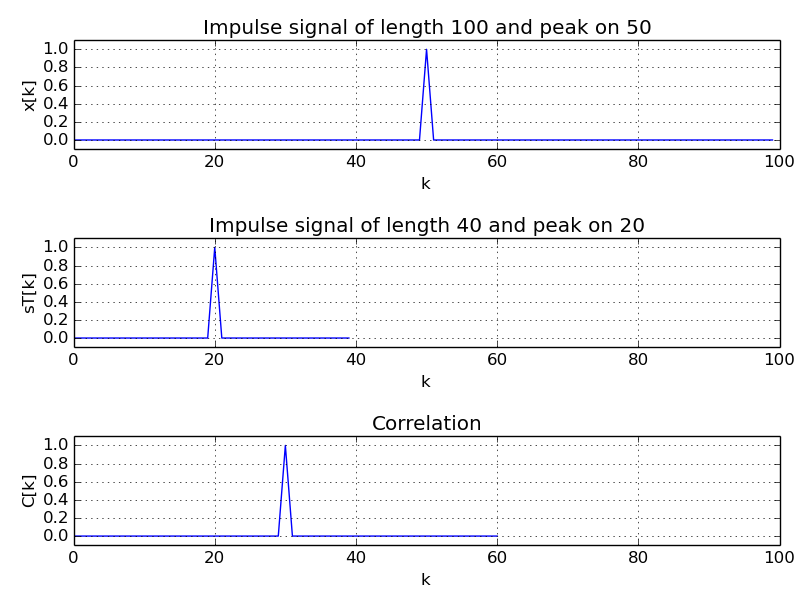
\includegraphics[width=\linewidth]{correlationOnImpulse.png}} \end{minipage}
    \caption{Cross correlation of 2 impulse signals}
    \label{correlationOnImpulse.png}
\end{figure}
The figure Fig\ref{correlationOnImpulse.png} shows that the result of the correlation of this two impulse signals is also an impulse signal.   Its non null value is the non null value $k_{x}^{0}$ of the first signal left shifted by the non null value $k_{s_{T}}^{0}$ of the second signal.   This statement can easily be explained thanks to the formula of the cross correlation: the value $l$ such as $C_{s_{T}, x}[l] \neq 0$ correspond to $x[k+l]*s_{T}[k] \neq 0$.   Thus 
\begin{itemize}
	\item $s_{T}[k] \neq 0 \rightarrow k = k_{s_{T}}^{0}$
    \item $x[k_{s_{T}}^{0}+l] \neq 0 \rightarrow$ $l = k_{x}^{0} - k_{s_{T}}^{0}$
\end{itemize}

Thanks to the program presented in the "Material \& Methods" section, we have also been able to observe the difference (indicator M) between $S_{T}$ and the shifted signals $x_{l}$.   This allowed as to confirm that this non null index of the correlation is also the index $l^*$ that maximizes $M(x_{l}, s_{T})$
    
    




	\subsubsection{Matching a more complex signal: Gaussian noise}
    Let now consider the periodic signal "$period$" defined in the "Material \& Methods" section.  Let suppose that this signal has been added to a Gaussian noise signal to create the input signal x.   Our objective is to match the input signal "$period$" into the perturbed signal x.   Thus we used our implemented algorithms to compute the cross correlation (hence the indicator M) of the x and the target signal.
\begin{figure}[!htb]\centering
    \begin{minipage}{0.49\textwidth} \frame{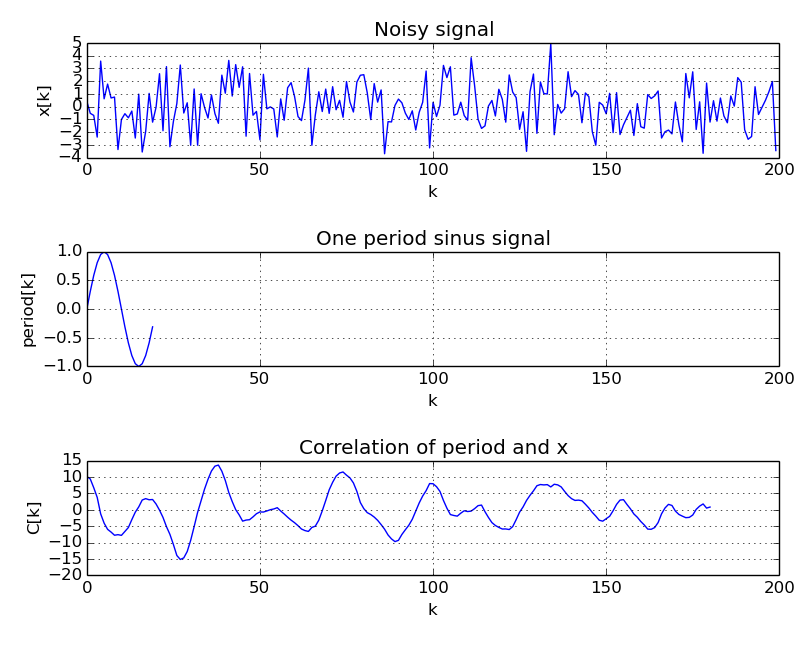
\includegraphics[width=\linewidth]{correlationOnSinAndNoise.png}} \end{minipage}
    \caption{Cross correlation of 2 impulse signals}
    \label{correlationOnImpulse.png}
\end{figure}
In the figure \ref{correlationOnImpulse.png} we can observe the result of this cross correlation computation is most of the time far from one.   Our "$argmax$" program confirmed this fact as it returned a value $C^* = max(M(x_{l}, s_{T})) = 0.175$.
This result means that for all the sub signal $x_{l}$ the difference between the sub signal and the target signal is too big to recognize any matching (too far from 1).   Thus, we can say that the Gaussian perturbation that we have introduced to our periodic signal has "modified the signal so much" that it can not be recognized by our "pattern matching method".   We have reached the limits of our method.  



    
    \subsection{Generalizing to a 2D-signal: Finding Waldo}
In order to find Waldo we tried to apply the same correlation method that we used before. However, as images are 2D signals some changes have to be made. We used \textit{correlate2D} image from the \textit{scipy.signal} package instead of \textit{correlate}. After it we tried to find the maximum of values inside the correlation matrix and check if Waldo is in this place. Without a doubt, this try was wrong and the location was random. After we looked at the values of the correlation matrix, we realized that they are in boundaries between 0 and 255 which was strange. Moreover, more than 1000 pixels have the maximum value of 255. In fact, the correlation was calculated using module of 255 as value of images can be more than 255. This was fixed just by changing type of matrix to float. However, even after the transformation, the maximum value of correlation was still not in the right place and we could not find Waldo. The matrix we got is shown in the figure \ref{correlate2D_first.png}, expected location of Waldo is shown as red square.\\\\
\begin{figure}[ht!]
	\label{correlate2D_first.png}
	\center
	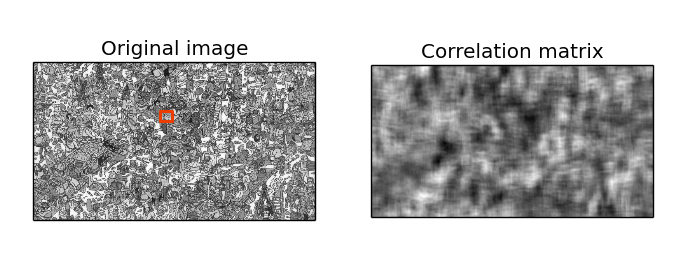
\includegraphics[width=0.8\linewidth]{img_double_1_edited.png}
	\caption{Original image and correlation matrix obtained by incorrect method}
\end{figure}
On this point we tried to implement method which was equivalent to the correlation formula for 1D signals proposed by \ref{M_equal_C} formula. The main difficulty here was to understand what $x'$ and $s'_T$ are. We came to an idea that we should use subimage of the original image with the size of the pattern as $x$ and the whole pattern as $s_T$. $s'_T$ is the same for every point of the correlation matrix and can be calculated as $\frac{s_T}{\sqrt{E(s_T)}}$. However $x'$ can change in every point as energies of different subimages are different. The idea was to calculate energy of every subimage and make the adjustment for the calculations. An efficient way to do it was to calculate the integral image of squares where  $I_{\sum}(x,y) = \sum_{\begin{smallmatrix} x' \le x \\ y' \le y\end{smallmatrix}} i(x',y')$. Applying dynamic programming, it can be done in $O(height*width)$ time. Than we can efficiently calculate $E(x, y) = I(x, y) + I(x + width, y + height) - I(x, y + height) - I(x + width, y)$ using only a few operations. As soon as we know how to quickly calculate $E(x)$ and $E(s_T)$, we can calculate the correlation matrix and than divide every value of it by corresponding energies. The results of such method is shown in the figure \ref{correlate2D_second.png}.\\\\
\begin{figure}[ht!]
	\label{correlate2D_second.png}
	\center
	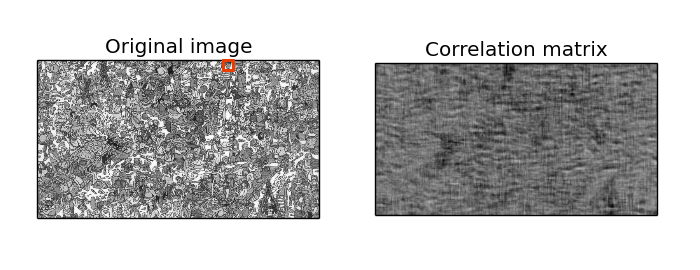
\includegraphics[width=0.8\linewidth]{img_double_2_edited.png}
	\caption{Original image and correlation matrix obtained by correct method}
\end{figure}
The same method was applied for the second image of Waldo. Results are represented in the image \ref{waldo_second.png} \textbf{TODO}. Write here that our method fucked up a bit.











\section{Conclusion}
Template matching technique presented in this report has its own advantages such as simplicity of understanding and implementation. \textbf{TODO}







\end{document}
